%************************************************
% Implementierung
%************************************************
\chapter{Implementierung}
\label{sec:implementation}

In diesem Kapitel wird die Implementierung des im Rahmen dieser Arbeit entwickelten Programms dargestellt, sowie die technischen Entscheidungen, die zu ihr geführt haben, erläutert. Außerdem beschreibt dieses Kapitel die Integration des entstandenen Tools in BlattWerkzeug.

%************************************************
% Rahmenhandlung
%************************************************
\section{Rahmenhandlung}
\label{sec:implementation:story}

Für die Festlegung einer Rahmenhandlung bieten sich im wesentlichen zwei Vorgehensweisen an:

\begin{enumerate}[noitemsep]
  \item Es wird zunächst eine Logik entwickelt und teilweise bereits implementiert. Die Rahmenhandlung wird erst später festgelegt und richtet sich nach den gewünschten und ggf. implementierten Funktionen. Mit dieser Vorgehensweise lässt sich die Logik noch klarer von der Darstellung trennen. Die Darstellung wird austauschbar und es ist sogar denkbar, verschiedene Rahmenhandlungen auf derselben Logik zu implementieren. Ob in der endgültigen Rahmenhandlung nun also Roboter oder Marienkäfer vom Programm gesteuert werden, wird erst definiert, wenn die Struktur der Programme festgelegt wurde.
  \item Eine andere Vorgehensweise ist es, die Rahmenhandlung direkt am Anfang festzulegen. Die Anforderungen der Rahmenhandlung diktieren in diesem Fall die Logik. Naturgemäß fließen Anforderungen an die Logik bei der Festlegung der Rahmenhandlung auch hier mit ein. Allerdings sind Darstellung und Logik bei dieser Vorgehensweise viel enger aneinander geknüpft. Ein späteres Austauschen der Darstellung wird deutlich erschwert. Die engere Verbindung bedeutet allerdings auch eine bessere Abstimmung der beiden Komponenten.
\end{enumerate}

Für diese Arbeit wurde die zweite Vorgehensweise gewählt, um so die Minisprache besser auf die Rahmenhandlung abstimmen zu können, und im ersten Schritt unter Berücksichtigung der Anforderungen an die Logik eine Entscheidung über eine Rahmenhandlung getroffen. Das Ziel ist es, mithilfe eines Lastwagens, welcher vom Spieler über Programmbefehle steuerbar ist (siehe \ref{sec:requirements:program}), über ein Netz von Straßen, verschiedenfarbige Container an ihre vorgesehenen Ablageorte zu bringen. Dabei ist die Ladefläche des Lastwagens auf einen Container begrenzt, womit unter Umständen zur Lösung mehrfache Fahrten -- auch Teilfahrten -- notwendig werden können. Dargestellt wird die Mikrowelt in einer Überkopf-Ansicht, wie sie aus Turtle Grafiken, Karel und Kara bekannt ist. Damit kann der Nutzer das Straßennetz schnell erfassen und sich die möglichen Wege zum Ziel überlegen.

Diese Rahmenhandlung wurde gewählt, da der Transport von Waren in dieser vereinfachten Darstellung allgemein bekannt sein dürfte und sich die Nutzer gut in die Rolle des Fahrers hineinversetzen können. In Zeiten, in denen autonomes Fahren ein viel diskutiertes Thema ist, gewinnt diese Rahmenhandlung zusätzlich an Relevanz. Außerdem bietet sie verschiedene Erweiterungsmöglichkeiten, durch die eine schrittweise Erhöhung der Komplexität erreicht werden kann. So ermöglicht die Einführung von Verkehrsampeln z.~B. die Vermittlung des Konzeptes der Verzweigungen und zeitlicher Zusammenhänge.

%************************************************
% Objektstruktur
%************************************************
\section{Objektstruktur}
\label{sec:implementation:structure}

Es wurde zunächst eine objektorientierte Datenstruktur erarbeitet, die eine Welt repräsentiert und Methoden bereitstellt, welche Operationen auf dieser Welt durchführen können. Abbildung \ref{fig:implementation:structure:uml} zeigt ein UML-Diagramm dieser Struktur. Zur besseren Übersicht wurde diese Darstellung auf die wesentlichen, zum Verständnis notwendigen Klassen, Attribute und Operationen beschränkt.

\begin{figure}
  \begin{tikzpicture}
  \tikzstyle{every node}=[font=\small]

  \begin{class}[text width=5cm]{World}{4.75,0}
    \attribute{commands}
    \attribute{sensors}

    \operation{command(command: Command)}
    \operation{sensor(sensor: Sensor): boolean}
  \end{class}

  \begin{class}[text width=3cm]{Size}{-1.5,-1}
    \attribute{width: number}
    \attribute{height: number}
  \end{class}

  \begin{class}[text width=3cm]{WorldState}{11,-1.5}
    \attribute{step: number}
    \attribute{time: number}
    \attribute{prev: WorldState}
  \end{class}

  \begin{class}[text width=4cm]{Tile}{-1,-3.5}
    \attribute{position: Position}
    \attribute{freightTarget: Freight}

    \operation{addFreight(freight: Freight)}
    \operation{removeFreight(): Freight}
  \end{class}

  \begin{class}[text width=5cm]{Truck}{10,-5}
    \attribute{position: Position}
    \attribute{facing: number}

    \operation{loadFreight(freight: Freight)}
    \operation{unloadFreight(): Freight}
    \operation{turn(turnDirection: TurnDirection)}
    \operation{move()}
  \end{class}

  \begin{class}[text width=6cm]{TrafficLight}{4.75,-10}
    \attribute{redPhase: number}
    \attribute{greenPhase: number}
    \attribute{initial: number}

    \operation{isRed(step: number): boolean}
    \operation{isGreen(step: number): boolean}
  \end{class}

  \begin{enumeration}[text width=4cm]{TileOpening}{-1,-8}
    \attribute{None}
    \attribute{North}
    \attribute{East}
    \attribute{South}
    \attribute{West}
  \end{enumeration}

  \begin{enumeration}[text width=3.5cm]{Freight}{4.25,-4.5}
    \attribute{Red}
    \attribute{Green}
    \attribute{Blue}
  \end{enumeration}

  \begin{enumeration}[text width=4cm]{TurnDirection}{10.5,-10.5}
    \attribute{Straight}
    \attribute{Left}
    \attribute{Right}
  \end{enumeration}

  \aggregation{World}{size}{1}{Size}
  \aggregation{World}{states}{*}{WorldState}
  \aggregation{WorldState}{tiles}{*}{Tile}
  \aggregation{WorldState}{truck}{1}{Truck}
  \aggregation{Tile}{trafficLights}{0..4}{TrafficLight}
  \unidirectionalAssociation{Truck}{turning}{1}{TurnDirection}
  \unidirectionalAssociation{Tile}{openings}{1..4}{TileOpening}
  \unidirectionalAssociation{Truck}{freight}{0..*}{Freight}
  \unidirectionalAssociation{Tile}{freight}{0..*}{Freight}
\end{tikzpicture}

  \caption{Vereinfachtes UML-Diagramm der Weltobjektstruktur}
  \label{fig:implementation:structure:uml}
\end{figure}

Wurzelelement dieser Struktur ist die \inlinec{World}-Klasse. Sie wird mit einer Beschreibung der zu generierenden Welt instanziiert. Anhand dieser Beschreibung erzeugt der Konstruktor die Größe (\inlinec{Size}) der Welt, einen Lastwagen (\inlinec{Truck}) und eine Menge von Kacheln (\inlinec{Tile}). Wobei die Kacheln Straßen repräsentieren wiederum Frachten und Ampeln beinhalten können. Lastwagen und Kacheln werden in einem Weltzustand (\inlinec{WorldState}) verpackt. Die Daten eines einmal gespeicherten Zustandes werden nicht mehr geändert. Stattdessen wird eine Kopie des aktuellen Zustandes erzeugt, verändert und in der Liste aller Zustände abgespeichert. Dieses Vorgehen ermöglicht dem Nutzer, Operationen rückgängig zu machen. Außerdem wird dadurch, die für die Animationen \tref{sec:implementation:rendering:animation} notwendige Interpolation zwischen Zuständen vereinfacht. Die Veränderung der Zustände übernimmt die \inlinec{World}-Klasse in der Operation \inlinec{command}. Da alle Operationen auf der Welt parameterlos sind, wird der \inlinec{command}-Methode lediglich der Name der auszuführenden Operation übergeben. Eine Liste der verfügbaren Befehle findet sich in Tabelle \ref{tbl:implementation:elements:cmds} auf Seite \pageref{tbl:implementation:elements:cmds}.

%************************************************
% Elemente der Minisprache
%************************************************
\section{Elemente der Minisprache}
\label{sec:implementation:elements}

Im Folgenden sind die Elemente beschrieben, welche dem Nutzer zum Programmieren innerhalb der bereitgestellten Umgebung zur Verfügung stehen.

\subsection*{Atomare Befehle}
\label{sec:implementation:elements:cmds}

Wichtigster Bestandteil sind die atomaren Befehle. Durch die Aneinanderreihung mehrerer Befehle lässt sich bereits ein sinnvolles Programm implementieren. Es wurden die in Tabelle \ref{tbl:implementation:elements:cmds} implementiert. Der Umfang orientiert sich im Wesentlichen an dem von JavaScriptKara (siehe Abbildung \ref{fig:related:kara:code}), wurde aber um weitere Befehle erweitert, deren Notwendigkeit bei Tests identifiziert wurde.

\begin{table}
  \begin{tabular}{|p{0.175\textwidth}|p{0.175\textwidth}|p{0.56\textwidth}|}
    \hline
    \textbf{Befehl} & \textbf{Interne\newline Repräsentation} & \textbf{Beschreibung} \\ \hline
    Vorwärts fahren & \inlinec{goForward} & Bewegt den Lastwagen nach vorne. Falls dabei ein Blinker in eine Richtung gesetzt ist, biegt der Lastwagen in die entsprechende Richtung ab. \\ \hline
    Blinker\newline links setzen & \inlinec{turnLeft} & Setzt den Blinker auf der linken Seite. Dadurch biegt der Lastwagen bei der nächsten Vorwärtsbewegung links ab. \\ \hline
    Blinker\newline rechts setzen & \inlinec{turnRight} & Setzt den Blinker auf der rechten Seite. Bei der nächsten Vorwärtsbewegung biegt der Lastwagen dadurch entsprechend rechts ab. \\ \hline
    Blinker\newline ausschalten & \inlinec{noTurn} & Schaltet einen zuvor gesetzten Blinker wieder aus. Dies ist nicht notwendig nach der Fahrt um eine Kurve, da sich der Blinker hier selbst ausschaltet, allerdings kann so ein "versehentliches" Setzen des Blinkers rückgängig gemacht werden. Dieser Befehl ist vor allem für die Bedienung im Navigationsmodus, da hier ein versehntlicher Klick leicht vorkommen kann. \\ \hline
    Aufladen & \inlinec{load} & Lädt ein Frachtstück, welches vor dem Lastwagen auf der Straße liegt, auf. \\ \hline
    Abladen & \inlinec{unload} & Lädt ein Frachtstück auf eine Ablagefläche oder einem leeren Streckenabschnitt vor dem Lastwagen wieder ab. \\ \hline
    Warten & \inlinec{wait} & Wartet einen Zeitschritt ab. Dieser Befehl ist wichtig, um das Warten an einer Ampel zu ermöglichen. \\ \hline
    Pause & \inlinec{pause} & Pausiert die Ausführung des Programms bis sie durch den Benutzer fortgesetzt wird. Diese Funktion dient als eine Art Breakpoint. Der Nutzer bekommt die Möglichkeit, sein Programm mit diesem Befehl zu pausieren und so z.~B. den Wert der Sensoren zu kontrollieren. Eine Art Debugging wird so ermöglicht. \\ \hline
  \end{tabular}
  \vspace{5pt}
  \caption{Atomare Befehle}
  \label{tbl:implementation:elements:cmds}
\end{table}

Bewegungen finden dadurch immer relativ zur aktuellen Blickrichtung des Lastwagens statt. Absolute Bewegungen mit Befehlen wie "Fahre nach Norden", "Fahre nach Osten" usw. sind vor allem aus Arcadespielen wie Pac-Man bekannt und haben den Vorteil, dass sich die Richtungen mit der Blickrichtung des Lastwagens nicht ändern und der Nutzer vor dem Bildschirm nicht umdenken muss. Relative Bewegungen hingegen lassen sich im Kontext von Programmierten Befehlen vielseitiger einsetzen. So kann eine Fahrt im Kreis z.~B. mit zwei Befehlen realisiert werden, welche in einer Schleife ausgeführt werden. Auch wurde dieser Ansatz den absoluten Bewegungen vorgezogen, da er der intuitiven Steuerungsart eines Lastwagens am nächsten kommt. Außerdem können daraus Vorteile für die Darstellung gewonnen werden, wie Abschnitt \ref{sec:implementation:rendering:truck-position} zeigt.

Der "Vorwärts fahren"-Befehl wurde zunächst mit einer gewissen Intelligenz ausgestattet. Dadurch konnten Kurven gefahren werden, ohne dass ein Blinker gesetzt werden musste. Im Laufe der Arbeit wurde diese Logik als eine mögliche Aufgabenstellung identifiziert und daher deaktiviert. Nutzer sollten sich eine Funktion definieren, die eben diesen intelligenten "Vorwärts fahren"-Befehl umsetzt.

\subsection*{Zählerschleife}
\label{sec:implementation:elements:for}

Um Codeverdoppelung zu vermeiden, kann eine Schleife eingesetzt werden, die einen Befehlsblock wiederholt. Die Anzahl der Wiederholungen kann vom Nutzer vorab festgelegt werden, ein vorzeitiges Verlassen der Schleife ist anschließend jedoch nicht mehr möglich. Damit ist es z.~B. möglich, für eine Fahrt auf einer langen Geraden den "Vorwärts fahren"-Befehl viermal in der Schleife auszuführen und ihn so nicht viermal im Programm wiederholen zu müssen.

\subsection*{Sensoren}
\label{sec:implementation:elements:sensors}

Um Verzweigungen nutzen zu können, gibt es die Möglichkeit Werte von Sensoren abzufragen. Sensoren geben einen booleschen Wert zurück, stehen also immer entweder auf wahr oder falsch. Tabelle \ref{tbl:implementation:elements:sensors} listet die zur Verfügung stehenden Sensoren auf. Auch hier orientiert sich der Umfang an JavaScriptKara und wurde um Sensoren erweitert, welche bei Tests für diese Rahmenhandlung sinnvoll erschienen. Die verfügbaren Sensoren sind in Tabelle \ref{tbl:implementation:elements:sensors} dargestellt.

\begin{table}
  \begin{tabular}{|p{0.175\textwidth}|p{0.19\textwidth}|p{0.56\textwidth}|}
    \hline
    \textbf{Sensor} & \textbf{Interne\newline Repräsentation} & \textbf{Beschreibung} \\ \hline
    Ampel ist rot & \inlinec{lightIsRed} & Dieser Sensor ist wahr, wenn die Ampel vor dem Lastwagen rot ist. Ist die Ampel grün oder gibt es keine Ampel vor dem Lastwagen, so steht dieser Sensor auf falsch. \\ \hline
    Ampel ist grün & \inlinec{lightIsGreen} & Analog dazu ist dieser Sensor wahr, wenn die Ampel vor dem Lastwagen grün ist und falsch, wenn sie auf rot steht oder es keine Ampel vor dem Lastwagen gibt. \\ \hline
    Kann geradeaus fahren & \inlinec{canGoStraight} & Dieser Sensor wertet zu wahr aus, wenn das Straßennetz es zulässt, dass der Lastwagen im nächsten Schritt geradeaus fahren kann. \\ \hline
    Kann links abbiegen & \inlinec{canTurnLeft} & Dieser Sensor wertet zu wahr aus, wenn im nächsten Schritt links abgebogen werden kann. \\ \hline
    Kann rechts abbiegen & \inlinec{canTurnRight} & Wenn im nächsten Schritt nach rechts abgebogen werden kann, wertet dieser Sensor zu wahr aus. \\ \hline
    Kann aufladen & \inlinec{canLoad} & Wenn auf der Kachel, auf welcher sich der Lastwagen aktuell befindet, aufgeladen werden kann, wertet dieser Sensor zu wahr aus. Das beinhaltet, dass der Lastwagen leer ist und sich auf der Kachel ein Container befindet. \\ \hline
    Kann abladen & \inlinec{canUnload} & Wenn auf der Kachel, auf welcher sich der Lastwagen aktuell befindet, abgeladen werden kann, wertet dieser Sensor zu wahr aus. Das beinhaltet nicht nur Ablageflächen, sondern auch leere Kacheln. \\ \hline
    Ist auf Ziel & \inlinec{isOnTarget} & Wenn sich die Kachel, auf der sich der Lastwagen befindet, eine Ablagefläche befindet, wertet dieser Sensor zu wahr aus. Dabei wird die Ladung des Lastwagens nicht berücksichtigt. In Verbindung mit "Kann abladen" kann z.~B. festgestellt werden, ob auf der Ablagefläche auch wirklich abgeladen werden kann. \\ \hline
    Ist gelöst & \inlinec{isSolved} & Wenn die aktuelle Welt gelöst wurde, also alle Frachtstücke zu ihren Zielen transportiert wurden, wertet dieser Sensor zu wahr aus. \\ \hline
  \end{tabular}
  \vspace{5pt}
  \caption{Sensoren}
  \label{tbl:implementation:elements:sensors}
\end{table}

\subsection*{Kopfgesteuerte Schleife}
\label{sec:implementation:elements:while}

Mit den Sensoren ist es möglich, eine kopfgesteuerte Schleife zu nutzen. Diese wiederholt den Befehlsblock solange der angegebene Ausdruck zu wahr auswertet. Wird die Schleifenbedingung vor der ersten Ausführung des Schleifenblocks oder nach ein oder mehreren Ausführungen zu falsch ausgewertet, wird der nachfolgende Block ausgeführt. Der Schleifenblock kann also auch komplett übersprungen werden.

Mit diesem Element kann z.~B. das Warten auf eine Ampel realisiert werden, wobei die Schleife immer wieder den "Warten"-Befehl ausführt, bis die Bedingung, dass die Ampel grün ist, erfüllt ist.

\subsection*{Verzweigungen}
\label{sec:implementation:elements:if-else}

Sensoren ermöglichen außerdem Verzweigungen, die einen Befehlsblock nur dann ausführen, wenn der angegebene Sensor zu wahr ausgewertet wird und einen weiteren, optionalen Befehlsblock, wenn der Sensor zu falsch ausgewertet wird.

Das aus anderen Sprachen bekannte \inlinec{elseif} gibt es, wie auch in JavaScript, in der hier definierten Sprache nicht. Um dieses Verhalten zu erreichen, müssen mehrere \inlinec{if...else}-Anweisungen geschachtelt werden.

In Zukunft wäre es denkbar, in dieser Form geschachtelte Verzweigungen auch im generierten Code ohne zusätzliche geschweifte Klammern und Einrückungen darzustellen. Bisher wurde auf diese Darstellung verzichtet, da auch der Drag \& Drop-Editor hierzu noch nicht in der Lage ist.

\subsection*{Logische Operatoren}
\label{sec:implementation:elements:op}

Unter Zuhilfenahme von logischen Operatoren können neue Ausdrücke erzeugt werden, welche sich wiederum in Schleifen und Verzweigungen einsetzen lassen.

\begin{itemize}[noitemsep]
  \item Die \emph{Nicht}-Operation kehrt den Wahrheitswert um.
  \item Die \emph{Und}-Verknüpfung ist wahr, wenn beide verknüpften Werte wahr sind.
  \item Die \emph{Oder}-Verknüpfung ist wahr, wenn mindestens einer der beiden verknüpften Werte wahr ist.
\end{itemize}

Mit diesen logischen Operatoren ist es nun z.~B. möglich, zu prüfen, ob das vorausliegende Streckenstück eine Kurve ist: (Kann nicht geradeaus fahren und ((Kann links abbiegen und Kann nicht rechts abbiegen) oder (Kann nicht links abbiegen und Kann rechts abbiegen)))

\subsection*{Prozeduren}
\label{sec:implementation:elements:proc}

Des Weiteren ist es möglich, eigene Prozeduren zu definieren und aufzurufen. Für Prozeduren lassen sich zusätzliche Parameter definieren, deren Nutzung innerhalb des Prozedurenblocks möglich ist. Jeder Parameter erhält einen vom Nutzer festgelegten Namen, kann jedoch ausschließlich boolesche Werte übergeben. Beim Aufruf der Prozedur werden die übergebenen Werte -- wie auch bei Prozeduraufrufen in JavaScript üblich -- kopiert.

Alle Prozeduren werden im Drag \& Drop-Editor in einem Deklarationsteil am Anfang des Programms definiert, da sich der Nutzer sonst zusätzliche Gedanken über den richtigen Ort der Deklaration machen müsste. Da Prozeduren deklariert werden müssen, bevor sie aufgerufen werden können, ist mit dieser Vorgehensweise sichergestellt, dass alle Prozeduren überall im Programm aufrufbar sind. Prozeduren sind auch in der Lage, sich selbst aufzurufen. Dies ermöglicht zusätzlich die Nutzung von Rekursion. In Verbindung mit Verzweigungen ist auch Rekursion mit Abbruchbedingung möglich.

Das im Abschnitt der kopfgesteuerten Schleife angesprochene Beispiel des Wartens auf Ampeln, ließe sich nun auch durch Rekursion lösen: Wenn die Ampel rot ist, führt sie den "Warten"-Befehl aus und ruft sich anschließend selbst wieder auf. Wird die Ampel grün, ist die Abbruchbedingung erfüllt und die Prozedur wird verlassen. Im Programm kann diese Funktionalität nun an verschiedenen Stellen wiederverwendet werden.

Im nächsten Schritt müssen die hier beschriebenen Elemente der Sprache in eine Grammatik übersetzt werden, nach welcher ein Syntaxbaum erzeugt werden kann. Diese Grammatik ist im nächsten Abschnitt beschrieben.

%************************************************
% Grammatik
%************************************************
\section{Grammatik}
\label{sec:implementation:grammar}

Im Grundlagenkapitel \ref{sec:basics:grammars} wurden bereits Aufbau und Funktionweise von Grammatiken in BlattWerkzeug erklärt. Es wird nun eine Grammatik definiert, welche die im vorherigen Abschnitt beschriebenen Elemente der Minisprache inkorporiert.

Wurzel der entwickelten Minisprache ist immer ein Programm, welches beliebig viele Prozedurdefinitionen (\inlinec{procedureDeclaration}), sowie mehrere Anweisungen (\inlinec{statement}) eines Hauptprogramms als Kindknoten aufnehmen kann. Prozeduren lassen sich nur in diesem Deklarationsteil definieren. Vom alternativen Vorgehen, Prozedurdefinitionen und Befehle im Hauptprogramm zu mischen, wurde abgesehen, damit der Nutzer seine Prozeduren später in jedem Teil seines Programms gleichermaßen verwenden kann und sich nicht explizit Gedanken, über die die Reihenfolge seiner Prozedurdefinitionen sein muss. Abbildung \ref{fig:implementation:grammar:1} zeigt den Einstieg in die Grammatik.

\begin{figure}[h]
  \lstinputlisting{snippets/implementation-program-grammar-syntaxtree-grammar-1.txt}
  \caption{Grammatik mit Programm-Knoten}
  \label{fig:implementation:grammar:1}
\end{figure}

Der Knoten zur Prozedurdefinition (\inlinec{procedureDeclaration}) ist in Abbildung \ref{fig:implementation:grammar:2} dargestellt. In  einer Eigenschaft wird der Name der Funktion angegeben. Eine Prozedur lässt sich mit Parametern (\inlinec{procedureParameter}) ausstatten und kann analog zum Hauptprogramm eine Liste von Anweisungen (\inlinec{statement}) als Kindknoten aufnehmen.

\begin{figure}[h]
  \lstinputlisting{snippets/implementation-program-grammar-syntaxtree-grammar-2.txt}
  \caption{Grammatik mit Prozedurdefinitions-Knoten}
  \label{fig:implementation:grammar:2}
\end{figure}

Eine Anweisung (\inlinec{statement}) kann ein Prozeduraufruf (\inlinec{procedureCall}), eine Verzweigung (\inlinec{if}), eine Zählerschleife (\inlinec{loopFor}) oder eine kopfgesteuerte Schleife (\inlinec{loopWhile}) repräsentieren. Mit einem Prozeduraufruf kann sowohl eine selbst definierte Prozedur als auch ein vorgegebener atomarer Befehl aufgerufen werden. Diese Entscheidung führt dazu, dass eigene Prozeduren und vorgegebene atomare Befehle im gleichen Geltungsbereich definiert sein müssen. Das beinhaltet, dass es möglich ist, mit eigenen Prozedurdefinitionen atomare Befehle zu überschreiben, bringt aber den Vorteil mit sich, dass Prozeduraufrufe einheitlich dargestellt werden können. Für einen Prozeduraufruf wird ein Name sowie optional eine Liste von Argumenten festgelegt. Da Sensoren lediglich boolesche Werte enthalten, sind auch als Typen für Prozedurparameter lediglich boolesche Werte (\inlinec{booleanExpression}) vorgesehen. Eine Erweiterung der Minisprache um ein Typsystem wäre jedoch für eine spätere Version denkbar, sodass z.~B. auch Integerwerte für Zählerschleifen übergeben werden können. Abbildung \ref{fig:implementation:grammar:3} zeigt die Definition von \inlinec{statement} und \inlinec{procedureCall}.

\begin{figure}[h]
  \lstinputlisting{snippets/implementation-program-grammar-syntaxtree-grammar-3.txt}
  \caption{Grammatik mit Prozeduraufruf-Knoten}
  \label{fig:implementation:grammar:3}
\end{figure}

Boolesche Werte (\inlinec{booleanExpression}) repräsentieren einen Sensor, einen invertierten Ausdruck, eine logische Verknüpfung oder eine boolesche Konstante. Sensoren (\inlinec{sensor}) haben die Eigenschaft \inlinec{type}, deren Wert aus der Liste der vorhandenen Sensortypen gewählt werden kann. Die Einschränkung, welche bei den Prozeduraufrufen aus den oben genannten Gründen nicht vorgenommen wurde, reduziert an dieser Stelle die Fehleranfälligkeit, bringt jedoch den Nachteil mit sich, dass neu hinzugefügte Sensoren zusätzlich eine Änderung der Grammatik erfordern. In Abbildung \ref{fig:implementation:grammar:4} sind diese Definitionen in der Grammatik dargestellt.

\begin{figure}[h]
  \lstinputlisting{snippets/implementation-program-grammar-syntaxtree-grammar-4.txt}
  \caption{Grammatik mit Knoten für boolesche Ausdrück und Sensoren}
  \label{fig:implementation:grammar:4}
\end{figure}

Invertierte Ausdrücke (\inlinec{negateExpression}) nehmen lediglich einen anderen booleschen Ausdruck auf. Dadurch ist z.~B. auch ein doppeltes Invertieren möglich. Logische Verknüpfungen (\inlinec{booleanBinaryExpression}) nehmen hingegen jeweils einen booleschen Wert für die linke und die rechte Seite, sowie einen Operator (\inlinec{relationalOperator}) auf (siehe Abbildung \ref{fig:implementation:grammar:5}).

\begin{figure}[h]
  \lstinputlisting{snippets/implementation-program-grammar-syntaxtree-grammar-5.txt}
  \caption{Grammatik mit Knoten für logische Operationen}
  \label{fig:implementation:grammar:5}
\end{figure}

Ein Knoten für Verzweigungen beinhaltet ein boolesches Prädikat (\inlinec{booleanExpression}) sowie Anweisungen (\inlinec{statement}) im Hauptteil und im alternativen \inlinec{else}-Teil. Dadurch werden mit nur einem Knoten alle Arten von Verzweigungen ermöglicht. Alternativ hätten auch zwei sperate Knoten für \inlinec{if}- und \inlinec{if...else}-Verzweigungen eingeführt werden können, oder einen \inlinec{if}-Knoten, der mehrere \inlinec{else if}-Knoten und höchstens einen \inlinec{else}-Knoten aufnehmen kann. Die Grammatik für Verzweigungen ist in Abbildung \ref{fig:implementation:grammar:6} dargestellt.

\begin{figure}[h]
  \lstinputlisting{snippets/implementation-program-grammar-syntaxtree-grammar-6.txt}
  \caption{Grammatik mit Knoten für Verzweigungen}
  \label{fig:implementation:grammar:6}
\end{figure}

Die Zählerschleife bekommt einen Integerwert als Eigenschaft, der angibt, wie oft die Schleife wiederholt werden soll. Auch hier wird über Kindknoten der Schleifenrumpf definiert. Abbildung \ref{fig:implementation:grammar:6} zeigt die Grammatik einer solchen Schleife.

\begin{figure}[h]
  \lstinputlisting{snippets/implementation-program-grammar-syntaxtree-grammar-7.txt}
  \caption{Grammatik mit Knoten für Zählerschleifen}
  \label{fig:implementation:grammar:7}
\end{figure}

Die Grammatik der kopfgesteuerten Schleife verfügt schließlich Kindknoten für ihr Prädikat, sowie ihren Schleifenrumpf und ist in Abbildung \ref{fig:implementation:grammar:8} dargestellt.

\begin{figure}[h]
  \lstinputlisting{snippets/implementation-program-grammar-syntaxtree-grammar-8.txt}
  \caption{Grammatik mit Knoten für kopfgesteuerte Schleifen}
  \label{fig:implementation:grammar:8}
\end{figure}

Aus dieser Grammatik ergibt sich ein Syntaxbaum, dessen Auswertung im nächsten Abschnitt beschrieben wird.

%************************************************
% Auswertung
%************************************************
\section{Auswertung}
\label{sec:implementation:evaluation}

Für die Auswertung und Ausführung des durch den Syntaxbaum beschriebenen Codes kommen zwei Vorgehensweisen infrage. In der Informatik bezeichnet der Begriff Kompilieren klassischerweise die Übersetzung von menschenfreundlichen Sprachelementen in maschinennahen Instruktionen, die von einem Prozessor und dem Betriebssystem verarbeitet werden können. Beim Interpretieren wird das Programm nicht vollständig übersetzt, sondern "portionsweise" analysiert, in eine zugehörige Folge von Prozessorinstruktionen übertragen und ausgeführt~\cite[47]{wagenknecht2009}. Da im Browser jedoch nicht direkt Maschinencode ausgeführt werden kann, ist der Unterschied in diesem Zusammenhang etwas anders zu verstehen:

\begin{itemize}
  \item Beim \emph{Interpretieren} wird der Syntaxbaum nach und nach durch ein in JavaScript geschriebenes Programm abgearbeitet und die entsprechenden Befehle direkt ausgeführt. In dieser Umgebung lässt sich der Fortschritt des Programms leicht verfolgen, da der Interpreter zu jedem Zeitpunkt die Position kennt, bis zu der der Code bisher ausgeführt wurde. Dies ermöglicht den Einbau von aussagekräftigen Debuggingfunktionen für den den auszuführenden Code. Außerdem ist es leicht möglich Mechanismen bereitzustellen, welche die Ausführung an einer beliebigen Stelle stoppen oder pausieren und später fortsetzen.
  \item Im Unterschied dazu ist \emph{Kompilieren} in diesem Zusammenhang so zu verstehen, dass ein JavaScript-Programm den Syntaxbaum zunächst in ein vollständig ausführbares JavaScript-Programm überführt. Der JavaScript-Code liegt bei diesem Vorgehen nach dem Kompilieren als String vor und kann anschließend als Ganzes in einer Art "Sandkasten" ausgeführt werden. Innerhalb dieser "Blackbox" lässt sich nur recht unzuverlässig auf den aktuellen Zustand des laufenden Programmes schließen ohne zusätzlichen Code einzufügen, der die Lesbarkeit des generierten Codes verschlechtert. Eben diese Lesbarkeit des generierten Codes ist aber einer der wichtigsten Vorteile dieser Vorgehensweise. Der Code lässt sich nicht nur für seine Ausführung nutzen, sondern kann gerade im Kontext einer Lernsoftware für den Nutzer interessant sein und ihm angezeigt werden.
\end{itemize}

Im Verlauf der Arbeit wurde die Vorgehensweise "Kompilieren" als Anforderung vorgegeben, da dieses Vorgehen speziell für BlattWerkzeug den Vorteil mit sich bringt, dass generierter Code in Zukunft vor der Ausführung dem Nutzer angezeigt und von ihm bearbeitet werden kann, was den Übergang zu einer Universalsprache erleichtern würde (siehe auch \ref{sec:conclusion:future}).

\subsection{Codegenerator}
\label{sec:implementation:evaluation:codegenerator}

Für die Kompilierung des Syntaxbaumes wird auf die von BlattWerkzeug zur Verfügung gestellten Codegenerator-Strukturen zurückgegriffen, die es ermöglichen, einen Codegenerator zu implementieren, der Übersetzungsregeln für jeden Knotentyp definiert. Abbildung \ref{fig:implementation:evaluation:codegenerator} zeigt die Implementierung eines Codegenerators für Knoten, die eine While-Schleife repräsentieren. Zwischen den Klammern innerhalb der \inlinec{while}-Anweisung wird der Kindknoten für die Bedingung der Schleife eingefügt, gefolgt vom Inhalt der Schleife. Diese Kindknoten werden wiederum durch ähnlich aufgebaute Generatoren umgewandelt bis der vollständige Code des Wurzelknotens im Syntaxbaum übersetzt wurde. Abbildung \ref{fig:implementation:evaluation:tree-render} zeigt den Ausschnitt eines Syntaxbaumes, welcher durch den Codegenerator in den in Abbildung \ref{fig:implementation:evaluation:tree-result} gezeigten Code kompiliert wird.

\begin{figure}
  \lstinputlisting{snippets/implementation-program-evaluation-codegenerator.ts}
  \caption{Implementierung des Codegenrator für eine Verzweigung}
  \label{fig:implementation:evaluation:codegenerator}
\end{figure}

\begin{figure}
  \centering
  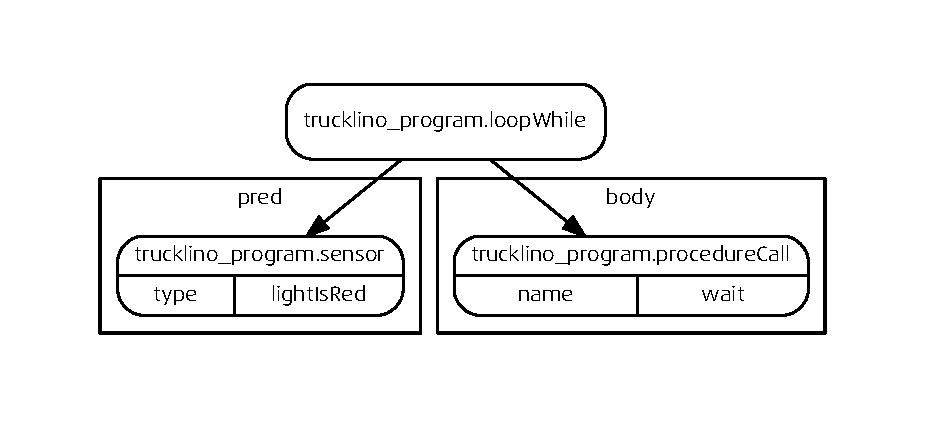
\includegraphics[width=\textwidth]{gfx/implementation-program-evaluation-tree.graphviz.pdf}
  \caption{Beispielhafter Ausschnitt eines Syntaxbaum für eine Verzweigung}
  \label{fig:implementation:evaluation:tree-render}
\end{figure}

\begin{figure}
  \lstinputlisting{snippets/implementation-program-evaluation-tree-result.js}
  \caption{Kompilierter Code für den Syntaxbaum in Abbildung \ref{fig:implementation:evaluation:tree-render}}
  \label{fig:implementation:evaluation:tree-result}
\end{figure}

\subsection[Umgebung zur Ausführung]{Umgebung zur Ausführung\protect\footnotemark}
\label{sec:implementation:evaluation:environment}

\footnotetext{Zum Verständnis dieses und folgender Abschnitte werden grundlegende Kenntnisse über die Konzepte von Promises, asynchronen Funktionen und Generatorfunktionen in JavaScript vorausgesetzt.}

Dem kompilierten Code muss zur Ausführung eine Umgebung bereitgestellt werden, welche die in Tabelle \ref{tbl:implementation:elements:cmds} gelisteten und als "atomaren Befehle" bezeichneten Funktionen, sowie Funktionen zur Ermittlung der Sensorwerte (siehe Tabelle \ref{tbl:implementation:elements:sensors}) zur Verfügung stellt. Für diese Aufgabe bietet sich der \inlinec{Function}-Konstruktor\footnote{\url{https://developer.mozilla.org/de/docs/Web/JavaScript/Reference/Global_Objects/Function}} an. Dieser Konstruktor transfomiert einen String in eine ausführbare JavaScript-Funktion. Im Gegensatz zu \inlinec{eval} ermöglicht der \inlinec{Function}-Konstruktor die Ausführung von Code im globalen Gültigkeitsbereich, was zu besseren Programmiergewohnheiten führt und eine effizientere Code-Minimierung ermöglicht~\cite{mdn-function}. In diesem speziellen Fall wird für die Ausführung des Codes der \inlinec{GeneratorFunction}-Konstruktor\footnote{\url{https://developer.mozilla.org/de/docs/Web/JavaScript/Reference/Global_Objects/GeneratorFunction}} verwendet (siehe dazu auch Abschnitt \ref{sec:implementation:rendering:animation}).

Für die Bereitstellung der Befehle und Sensoren werden im folgenden vier Varianten betrachtet. In Abbildung \ref{fig:implementation:environment} werden Implementationsbeispiele dieser Varianten einander gegenüber gestellt.

\begin{description}
  \item[1. Definition und Aufruf mit Enum-Klasse:] Eine Enum-Klasse mit allen Sensoren und Befehlen, sowie zwei Funktionen für deren Auswertung gibt es schon. Darauf aufbauend wäre eine nahe liegende Möglichkeit, diese Funktionen und die Enum-Klassen einfach in der Welt bereitzustellen. Ein deutlicher Vorteil dieser Lösung ist der geringe zusätzliche Implementierungsaufwand und die verbesserte Wartbarkeit. Kommen neue Befehle oder Sensoren dazu, stehen diese automatisch auch in der Umgebung zur Verfügung. Der generierte Code ist jedoch nicht intuitiv und sollte er dem Nutzer angezeigt werden, nicht besonders gut zu verstehen. Außerdem halten sich die Funktionsaufrufe nicht an gängige Muster, was den späteren Umstieg auf Universalsprachen erschweren könnte \fref{fig:implementation:environment:func}.
  \item[2. Definition und Aufruf mit \inlinec|call|:] Eine weitere denkbare Lösung ist es, ein Objekt mit allen benötigten Funktionen für Befehle und Sensoren zu erzeugen und dieses als Wert von \inlinec{this} innerhalb der Funktion zur Verfügung zu stellen. Selbstdefinierte Prozeduren werden innerhalb der Funktion ebenfalls als Kinder von \inlinec{this} definiert. Dieses Vorgehen hat den Vorteil, dass der Code deutlich intuitiver wird, als dies bei der vorgehend beschriebenen Variante der Fall wäre. Jedem Aufruf muss zwar ein \inlinec{this} vorangestellt werden, jeder Befehl hat aber seinen eigenen Funktionsaufruf. Der zusätzliche Implementierungsaufwand ist allerdings ein Nachteil dieser Variante. Es müssen in einem Objekt Wrapper-Funktionen für alle Befehle und Sensoren definiert werden. Kommt zu einem späteren Zeitpunkt ein Befehl oder ein Sensor hinzu, muss dieser zusätzlich auch an dieser Stelle hinzugefügt werden. Außerdem müssen selbst definierte Prozeduren mithilfe von Pfeilfunktionen\footnote{\url{https://developer.mozilla.org/de/docs/Web/JavaScript/Reference/Functions/Pfeilfunktionen}} definiert werden, damit der Bezug zum \inlinec{this} nicht verloren geht \fref{fig:implementation:environment:this}.
  \item[3. Definition und Aufruf über Parameter:] Auch wäre es möglich, alle Befehle und Sensoren als Parameter der Funktion zu definieren. Dadurch würde im Vergleich zur vorigen Variante die Notwendigkeit entfallen, \inlinec{this} vor jeden Aufruf zu stellen. Da die Wrapper-Funktionen in diesem Fall allerdings ebenfalls zusätzlich definiert werden müssen und die Zuordnung ihrer Namen fehleranfällig ist, birgt dieses Vorgehen abgesehen von dem etwas kompakteren Code, keine weiteren Vorteile \fref{fig:implementation:environment:param}.
  \item[4. Definition und Aufruf mit einem Objekt als Parameter:] Letztlich kommt auch eine Kombination der Varianten zwei und drei infrage, bei der alle Befehle und Sensoren in einem Objekt zusammengefasst werden. Im Vergleich zu Variante zwei muss das \inlinec{this} lediglich durch einen Variablennamen ersetzt werden. Dadurch ist es nun nicht zwingend erforderlich, Pfeilfunktionen für die Definition von benutzerdefinierten Prozeduren zu nutzen \fref{fig:implementation:environment:obj}.
\end{description}

Für den Einsatz in dieser Arbeit ist Variante vier am sinnvollsten, da so Wartbarkeit und Lesbarkeit des generierten Codes in einem angemessenen Verhältnis stehen. Außerdem werden Generatorfunktionen\footnote{\url{https://developer.mozilla.org/de/docs/Web/JavaScript/Reference/Statements/function*}} für die benuzterdefinierten Prozeduren verwendet, welche die Definition über Pfeilfunktionen nicht unterstützen. Der \inlinec{this}-Kontext würde bei Variante zwei dadurch verloren gehen.

Es wird also ein Objekt mit Wrapper-Funktionen für alle Befehle und Sensoren erzeugt und dieses als Parameter mit dem Namen \inlinec{truck} an die generierte Funktion übergeben. Die Bezeichnung \inlinec{truck} wurde gewählt, da alle Befehle aus Sicht des Trucks ausgeführt werden und \inlinec{truck.goForward()} sinnvoll lesbar sind.

\begin{figure}
  \begin{subfigure}[b]{\textwidth}
    \lstinputlisting{snippets/implementation-program-environment-func.js}
    \caption{Definition und Aufruf mit Enum-Klasse}
    \label{fig:implementation:environment:func}
    \vspace{0.5cm}
  \end{subfigure}
  \begin{subfigure}[b]{\textwidth}
    \lstinputlisting{snippets/implementation-program-environment-this.js}
    \caption{Definition und Aufruf mit \inlinec|call|}
    \label{fig:implementation:environment:this}
    \vspace{0.5cm}
  \end{subfigure}
  \begin{subfigure}[b]{\textwidth}
    \lstinputlisting{snippets/implementation-program-environment-param.js}
    \caption{Definition und Aufruf über Parameter}
    \label{fig:implementation:environment:param}
    \vspace{0.5cm}
  \end{subfigure}
  \begin{subfigure}[b]{\textwidth}
    \lstinputlisting{snippets/implementation-program-environment-obj.js}
    \caption{Definition und Aufruf mit einem Objekt als Parameter}
    \label{fig:implementation:environment:obj}
  \end{subfigure}
  \caption{Varianten für die Bereitstellung der Befehle und Sensoren innerhalb der generierten Funktion}
  \label{fig:implementation:environment}
\end{figure}

\subsection{Ausführungsdauer von Befehlen}
\label{sec:implementation:evaluation:execution-time}

Die Ausführung der atomaren Befehle wie dem des Vorwärtsfahren oder Warten haben in JavaScript aufgrund ihrer geringen Komplexität eine kaum merkliche Ausführungszeit. Um die Ausführung trotzdem sichtbar zu machen, soll diese Ausführungszeit künstlich erhöht werden können. Diese Eigenschaft ist unter anderem auch für die Animation in der Darstellung (siehe \ref{sec:implementation:rendering:animation}) von Bedeutung.

Zur Darstellung einiger Operationen wird eine gewisse Zeit benötigt. So ist für die Operation des Vorwärtsfahrens, ein Zeitschritt festgelegt, beim Setzen eines Blinkers kann die verbrauchte Zeit jedoch vernachlässigt werden, daher wird diese Operation mit null Zeitschritten bewertet. Die tatsächliche Zeit, die ein Zeitschritt verbraucht, kann separat festgelegt werden. Dadurch ist es möglich die Zeit (z.~B. für die Auswertung von Testfällen) kleiner zu stellen und dadurch die Ausführung schneller laufen zu lassen.

Auch sind die Zeitschritte für die Berechnung der Ampelphasen relevant. Für Ampeln kann die Dauer der Rot- und Grünphasen in Zeitschritten festgelegt werden. Eine Ampel mit einer Rotphase von einem Zeitschritt sowie einer Grünphase von ebenfalls einem Zeitschritt wird nun nach jeder Vorwärtsbewegung oder Aufruf des Warten-Befehls umspringen, jedoch nicht beim Wechsel der Blinkerseite.

Um der Ausführungszeit im Programmablauf gerecht zu werden, stellt die \inlinec{World}-Klasse neben der \inlinec{command}-Methode zusätzlich die Methode \inlinec{commandAsync} bereit, die als asynchrone Funktion definiert ist und ein \inlinec{Promise} zurückgibt, welches erfüllt wird, sobald die für diesen Befehl vorgesehene Zeit abgelaufen ist.

Um auch das Pausieren und Fortsetzen der Ausführung zu ermöglichen, kommt für die Ausführung des generierten Codes eine Generatorfunktion zum Einsatz (siehe \ref{sec:implementation:evaluation:pause}).

\subsection{Behandlung von Endlosschleifen}
\label{sec:implementation:evaluation:infinite-loop}

Im Vergleich zu Beginn dieses Abschnittes, wurde ein Vorteil der Vorgehensweise "Interpretieren" genannt, welcher gleichzeitig ein Nachteil beim Kompilieren darstellt: Wurde mit der Ausführung des kompilierten Codes einmal begonnen, kann diese nicht einfach unterbrochen werden. Dies stellt insbesondere ein Problem dar, wenn der Nutzer eine Endlosschleife in sein Programm eingebaut hat. Das Programm läuft im gleichen Kontext wie die Webseite und kann diese daher einfrieren. Um dieses Problem zu umgehen, wurde zusätzlich der \inlinec{doNothing}-Befehl eingeführt. Dieser Befehl steht im Drag \& Drop-Editor nicht zur Verfügung. Er verändert -- ähnlich wie der \inlinec{wait}-Befehl -- den Zustand der Welt nicht, fügt im Gegensatz zu \inlinec{wait} allerdings keinen neuen Zustand ein, kann also auch nicht rückgängig gemacht werden. Trotzdem erzeugt dieser Befehl eine für den Nutzer kaum merkliche Wartezeit von wenigen Millisekunden. Mit diesem Vorgehen kann aktives Warten ("busy waiting") beim Aufruf einer leeren While-Schleife und daraus resultierendes Blockieren der Bedienelemente von BlattWerkzeug vermieden werden.

Den \inlinec{doNothing}-Befehl nur in leeren Schleifen einzufügen, reicht nicht aus. Zwar wäre es möglich, vereinzelte Konstellationen zu überprüfen und auf den zusätzlichen Befehl zu verzichten, wenn eine andere Anweisung auf gleicher Ebene aufgerufen wird, allerdings wird dieses Vorgehen sehr aufwendig, wenn auch kompliziertere Strukturen wie z.~B. Verzweigungen oder untergeordnete Schleifen geprüft werden sollen. Dabei handelt es sich um eine Variante des Halteproblems. Es kann in vielen Fällen nicht sichergestellt werden, dass ein bestimmter Codepfad auch wirklich aufgerufen und der darin enthaltene Befehl ausgeführt wird.

Im nächsten Schritt ist es möglich, das Programm innerhalb einer Endlosschleife manuell vorzeitig zu beenden, bzw. zu pausieren.

\subsection{Vorzeitiges Beenden der Ausführung}
\label{sec:implementation:evaluation:pause}

Für das vorzeitige Beenden des Programms schien zunächst die Variante sinnvoll, dass zusätzlich innerhalb von allen Befehlen geprüft wird, ob der Nutzer die Beendigung des laufenden Programmes angewiesen hat. Ist dies der Fall, wird die Ausführung des aktuellen Codes durch den Wurf einer Exception vorzeitig beendet. Dieses Vorgehen ist eine Möglichkeit, die Ausführung des Codes vorzeitig zu beenden, ohne die Lesbarkeit durch zusätzliche Kontrollbefehle zu verschlechtern, hat allerdings die Nebenwirkung, dass \inlinec{try...catch}-Anweisungen in Zukunft nicht innerhalb des generierten Codes eingesetzt werden können. Außerdem ist es mit diesem Verhalten nicht möglich, das Programm an der Stelle fortzuführen, an der es gestoppt wurde, da der Kontext der Funktion mit dem Wurf der Exception verloren geht.

Dieses Problem wird mit der Nutzung von Generatorfunktionen umgangen. Der erzeugte Iterator führt in jedem Iterationsschritt einen Befehl aus und gibt das \inlinec{Promise} zurück, auf dessen Erfüllung gewartet wird, bevor in einer Schleife der nächste Iterationsschritt aufgerufen wird. Dies geschieht solange, bis alle Befehle im Programm abgearbeitet sind oder ein Flag innerhalb der \inlinec{World}-Klasse gesetzt wird, dass das Programm im nächsten Schritt pausiert werden soll. Da der Iterator gespeichert wird, kann im Falle eines Pausierens, die Ausführung an der Stelle fortgesetzt werden, an der sie stehen geblieben ist.

Im generierten Code muss dadurch allerdings jedem Funktionsaufruf ein \inlinec{yield*} vorangestellt werden. Außerdem müssen benutzerdefinierte Prozeduren ebenfalls als Generatorfunktionen definiert werden.

Die in den vorigen Abschnitten besprochene Datenstruktur, sowie die Elemente der Sprache benötigen nun eine geeignete Darstellung, deren Implementierung im nächsten Abschnitt diskutiert wird.

\subsection{Syntaxfehler}
\label{sec:implementation:syntax-errors}

Es kann nicht garantiert werden, dass der Code, welcher vom Codegenerator erzeugt wurde, frei von Syntaxfehlern ist. Dies kann aus der Kompilierung eines unvollständigen Syntaxbaumes resultieren. So kann es z.~B. vorkommen, dass die Bedingung bei einer While-Schleife leer ist. JavaScript wirft bei der Erzeugung der Funktion einen \inlinec{SyntaxError}. Um diesen Fehler abzufangen, muss die Erzeugung der Funktion innerhalb einer try...catch-Anweisung\footnote{\url{https://developer.mozilla.org/de/docs/Web/JavaScript/Reference/Statements/try...catch}} stattfinden \fref{fig:implementation:evaluation:try-catch}.

\begin{figure}
  \lstinputlisting{snippets/implementation-program-evaluation-try-catch.js}
  \caption{Möglicher Syntaxfehler innerhalb des generierten Codes}
  \label{fig:implementation:evaluation:try-catch}
\end{figure}

%************************************************
% Darstellung
%************************************************
\section{Darstellung}
\label{sec:implementation:rendering}

Erst die Darstellung in einer Mikrowelt erweckt die Minisprache zum Leben. Im Folgenden wird die Implementierung der Darstellung der zuvor definierten Datenstruktur beschrieben.

\subsection{Technologie}
\label{sec:implementation:rendering:technology}

Als mögliche Technologien für die Darstellung und Animation der Welt im Browser wurden vier Ansätze evaluiert. Eine Übersicht der Eigenschaften findet sich in Tabelle \ref{tbl:implementation:rendering:technology}.

\begin{itemize}[noitemsep]
  \item Rendering über klassische \emph{HTML}-Elemente und Styling mittels CSS und Integration von nachgeladenen Bilddateien.
  \item Rendering mittels eines eingebetteten \emph{SVG}-Elements.
  \item Rendering mittels eines \emph{Canvas}-Elements und Integration von nachgeladenen Bilddateien.
  \item Einsatz von \emph{WebGL} für die Darstellung einer dreidimensionalen Welt.
\end{itemize}

WebGL ist als Technologie für diese Arbeit als zu mächtig einzustufen. Die Erstellung von dreidimensionalen Modellen hätte den Rahmen dieser Arbeit gesprengt und -- abgesehen von einer möglichen schöneren Darstellung -- im Vergleich zu den übrigen Technologien keinen nennenswerten Nutzen gehabt.

Rendering mittels HTML oder SVG hat den Vorteil, dass sie sehr von den Funktionen des Angular-Framework profitieren. Die Datenstruktur kann direkt an HTML und SVG-Elemente angebunden werden und Angular kümmert sich um die Aktualisierung des DOM. Dieses Vorgehen reduziert den Aufwand für die Implementierung des Renderers enorm. Zusätzlich bringt Angular nativ ein Animationsframework mit. Für die Implementierung eines Prototyps wurde das Rendering mittels eines SVG-Element gewählt, da es gegenüber einfachem HTML den Vorteil bietet, Grafiken direkt und ohne zusätliches Nachladen von Ressourcen integrieren zu können.

In der Implementierung des Prototyps erwies sich allerdings das Animationsframework als ein Nachteil dieser Technologie. Angular setzt an dieser Stelle auf ein zustandsbasiertes System. Eine Animation findet immer zwischen zwei definierten Zuständen statt. Zustände können bestimmte CSS Regeln angeben, zwischen denen bei einem Zustandswechsel interpoliert wird~\cite{angular-animations}. Dieses System ist mit den Anforderungen, die der im Rahmen dieser Arbeit behandelte Anwendungsfall stellt, nicht kompatibel. Für die Animation eines Lastwagens müsste vielmehr zwischen verschiedenen Positionen interpoliert werden. Diese variablen Positionen lassen sich nicht sinnvoll auf fest definierte Zustände in Angular abbilden. Es müssten Zustände für jede Position des Lastwagens in jeder Drehung definiert werden.

So setzt die aktuelle Version des Programms auf einen Renderer mittels Canvas-Element. Dass Angular keine Funktionen zum Rendern in einem Canvas-Element bereithält und dieser Prozess vollständig außerhalb und unabhängig von Angular stattfinden muss, erwies sich schnell als ein Vorteil dieser Technologie. Der Renderer hat dadurch keine externen Abhängigkeiten, ermöglicht eine leichte Integration in BlattWerkzeug und könnte potenziell auch in eine Anwendung portiert werden, welche Angular nicht einsetzt. Der Nachteil, dass das Canvas in jedem Frame vollständig neu gezeichnet werden muss, wäre technisch zu umgehen, indem Bereiche ermittelt werden, die sich im Vergleich zum letzten Frame geändert haben und nur diese Bereiche neu gezeichnet werden. Auf die Implementierung dieses Verhaltens wurde allerdings in diesem Fall verzichtet, da aufgrund der geringen Komplexität der zu zeichnenden Grafik zu erwarten ist, dass moderne Computer keinerlei Schwierigkeiten beim ständigen Neuzeichnen des Bildes haben werden und die angesprochene Technik nicht trivial umzusetzen ist.

\begin{table}
  \centering
  \begin{tabular}{l|c|c|c|c}
                                      & HTML   & SVG    & Canvas & WebGL  \\ \hline
    Direkte Integration in Angular    & \cmark & \cmark & \xmark & \xmark \\ \hline
    Frameweises Rendering             & \xmark & \xmark & \cmark & \cmark \\ \hline
    Nachladen von Ressourcen notwenig & \cmark & \xmark & \cmark & \cmark \\ \hline
    Abhängigkeitsfrei                 & \xmark & \xmark & \cmark & \cmark \\ \hline
    Komplexe 3D-Modellen notwendig    & \xmark & \xmark & \xmark & \cmark \\ \hline
  \end{tabular}
  \vspace{5pt}
  \caption{Vergleich der Darstellungstechnologien}
  \label{tbl:implementation:rendering:technology}
\end{table}

\subsection{Objektstruktur}
\label{sec:implementation:rendering:structure}

Für das effektive Zeichnen der Welt auf einem Canvas-Element wurde eine Renderer-Klasse mit einer am Besucher-Schema orientierten Objektstruktur entwickelt, welche die einzelnen Elemente der Objektstruktur der Welt (siehe \ref{sec:implementation:structure}) zeichnet.

Die Objektstruktur des Renderers ist in \figreft{sec:implementation:rendering:structure:uml} zur besseren Übersicht vereinfacht dargestellt. Wurzelklasse ist hier der Renderer, welcher mit einem \inlinec{World}-Objekt (diese Objektstruktur wurde in Abschnitt \ref{sec:implementation:structure} beschrieben) und einem Canvas-Context instanziiert wird. Mit dem Aufruf der \inlinec{render}-Methode wird der Render-Prozess gestartet. Diese Methode zeichnet den Canvas-Inhalt und ruft sich mittels der \inlinec{requestAnimationFrame}-Funktion\footnote{\url{https://developer.mozilla.org/en-US/docs/Web/API/window/requestAnimationFrame}} immer wieder selbst auf.

Die Eigentliche Zeichenaufgabe gibt die \inlinec{Renderer}-Klasse jedoch an einen Baum von \inlinec{ObjectRenderer}-Klassen ab, die für die Darstellung wesentlicher visueller Objekte zuständig sind. Die Struktur der \inlinec{ObjectRenderer} ist an der Weltobjektstruktur orientiert. Die \inlinec{Renderer}-Klasse hält eine Instanz eines \inlinec{WorldRenderer}, welcher die von ihm gehaltene \inlinec{WorldStateRenderer}-Instanz über Zustandsänderungen der Welt informiert. Der \inlinec{WorldStateRenderer} verwaltet genau eine \inlinec{TruckRenderer}-Instanz, welche für das letztendliche Zeichnen des Lastwagens und die Animation von dessen Zustandsübergängen verantwortlich ist, sowie die notwendige Anzahl von \inlinec{TileRenderer}-Instanzen. Die \inlinec{draw}-Methode der \inlinec{ObjectRenderer} werden immer mit einem \inlinec{RenderingContext} aufgerufen, welcher den Zeitstempel der Animation verwaltet, einen Verweis auf den zu verwendenden Canvas-Context enthält, sowie einige Hilfsmethoden zum Zeichnen bereitstellt.

Das sichtbare Bild wird durch die \inlinec{ObjectRenderer} vollständig aus verschiedenen Komponenten zusammengesetzt, die aus SVG-Sprites an die richtige Stelle im Bild gezeichnet werden. Die Hintergründe der Straßen stammen aus einer freien Sammlung von Spielegrafiken\footnote{\url{https://opengameart.org/node/16589}}, der Truck und die Fracht wurden für den Zweck dieser Arbeit selbst gezeichnet. Alle 16 Varianten von Kacheln sind im Sprite verfügbar. Lediglich der Truck muss vor dem Zeichnen in die richtige Richtung gedreht werden. Ein Vorbereiten aller möglichen Drehungen des Lastwagens im Sprite ist an dieser Stelle nicht sinnvoll, da die Drehung des Lastwagens animiert interpoliert werden soll.

\begin{figure}
  \begin{tikzpicture}
  \tikzstyle{every node}=[font=\small]

  \begin{class}[text width=7cm]{Renderer}{1,0}
    \attribute{running: boolean}

    \operation{constructor(world: World, ctx: CanvasContext)}
    \operation{stop()}
    \operation{render(timestamp: TimeStamp)}
  \end{class}

  \begin{class}[text width=5cm]{RenderingContext}{9,0}
    \attribute{ctx: CanvasRenderingContext2D}
    \attribute{width: number}
    \attribute{height: number}
    \attribute{start: TimeStamp}
    \attribute{previousFrame: TimeStamp}
    \attribute{currentFrame: TimeStamp}

    \operation{animationSpeed(): number}
  \end{class}

  \begin{interface}[text width=5cm]{ObjectRenderer}{3.5,-3}
    \operation{draw(ctx: RenderingContext)}
  \end{interface}

  \begin{class}[text width=3cm]{WorldRenderer}{-1,-5}
    \implement{ObjectRenderer}

    \attribute{world: World}

  \end{class}

  \begin{class}[text width=4cm]{WorldStateRenderer}{-0.5,-7.5}
    \implement{ObjectRenderer}

    \attribute{state: WorldState}
    \attribute{freightTarget: Freight}

    \operation{update(state: WorldState)}
  \end{class}

  \begin{class}[text width=2.75cm]{TileRenderer}{5.5,-6}
    \implement{ObjectRenderer}

    \attribute{tile: Tile}

    \operation{update(tile: Tile)}
  \end{class}

  \begin{class}[text width=3.5cm]{TruckRenderer}{9.75,-7}
    % \implement{ObjectRenderer}

    \attribute{truck: Truck}
    \attribute{prevTruck: Truck}
    \attribute{initial: number}

    \operation{update(truck: Truck)}
  \end{class}

  \composition{Renderer}{ctx}{1}{RenderingContext}
  \composition{Renderer}{worldRenderer}{1}{WorldRenderer}
  \composition{WorldRenderer}{stateRenderer}{1}{WorldStateRenderer}
  \composition{WorldStateRenderer}{truckRenderer}{1}{TruckRenderer}
  \composition{WorldStateRenderer}{tileRenderers}{0..*}{TileRenderer}

  \draw[umlcd style implement line](ObjectRenderer) -- (TruckRenderer.north);
\end{tikzpicture}

  \caption{Vereinfachtes UML-Diagramm der Rendererobjektstruktur}
  \label{sec:implementation:rendering:structure:uml}
\end{figure}

\subsection{Zielerfüllung}
\label{sec:implementation:finish}

Hat der Nutzer mit seinem Programm oder aber manuell über die Befehlbuttons alle Container an ihr Ziel verbracht, erkennt die Software, dass das Spielfeld gelöst ist. Der Nutzer erhält eine Statusmeldung, dass das Spielfeld gelöst wurde, wird aber nicht aus der aktuellen Arbeitsumgebung herausgerissen. Vielmehr soll er die Möglichkeit bekommen, das eigene Programm noch einmal zu lesen und zu verstehen, \emph{warum} dieses Programm zu der Lösung geführt hat. Außerdem kann der Nutzer so sein Programm weiter optimieren und vielleicht eine Lösung implementieren, welche noch schneller zum gewünschten Ergebnis führt. Einzelne Schritte können dafür mithilfe eines entsprechenden Buttons rückgängig gemacht werden, oder aber die Welt wird direkt wieder auf ihren Ausgangszustand zurückgesetzt.

\subsection{Level-Editor}
\label{sec:implementation:level-editor}

Für den Drag \& Drop-Editor wurde eine weitere Grammatik in BlattWerkzeug eingeführt, welche es ermöglicht, eine eigene Karte zu kreieren. Der hieraus generierte Syntaxbaum wird in eine Beschreibung einer Welt (\inlinec{WorldDescription}) umgewandelt, mit der die \inlinec{World}-Klasse instanziiert werden kann. Abbildung \ref{fig:implementation:level-editor:tree} zeigt auschnittsweise einen beispielhaften Syntaxbaum für eine Welt. Diese Beschreibung enthält sowohl die Größe der Welt, sowie die Position und initiale Beladung des Lastwagens, als auch eine Liste von Kacheln, welche wiederum ihre Position definieren und Informationen über Ampeln, Fracht und Frachtziele enthalten.

Für die Aufgabe der Definition einer umfangreichen listenartigen Datenstruktur wie der einer Welt, erwies sich der Drag \& Drop-Editor als eher ungeeignet. Der Nutzer muss ein sehr genaues Bild der Welt vor Augen haben, um die Kacheln mit den richtigen Öffnungen zu platzieren. Um die Welten für die Beispielaufgaben besser erzeugen zu können, wurde ein rudimentärer Level-Editor entwickelt, der als JavaScript-Anwendung unabhängig von BlattWerkzeug funktioniert und den Syntaxbaum der Welt ausgibt. Dieser muss anschließend manuell in die BlattWerkzeug-Datenbank einkopiert werden. Da dies keine Lösung für reguläre Anwender darstellt und damit Lehrer ohne tiefer gehende Kenntnisse der Software in Zukunft selbst in der Lage sind, eigene Aufgabenstellungen vorzubereiten, wäre die Entwicklung eines geeigneten Level-Editors innerhalb der BlattWerkzeug-Umgebung, aber unabhängig vom Drag \& Drop-Editor, notwendig. In Absprache mit den Gutachtern wurde dieser Ansatz aus Zeitgründen nicht weiter verfolgt.

\begin{figure}
  \lstinputlisting{snippets/implementation-program-level-editor-tree.json}
  \caption{Beispielhafter Syntaxbaum einer Welt (verkürzt)}
  \label{fig:implementation:level-editor:tree}
\end{figure}

\subsection{Lastwagen-Position}
\label{sec:implementation:rendering:truck-position}

Sowohl bei Kara \tref{sec:related:kara}, als auch bei Lightbot \tref{sec:related:lightbot} bewegt sich die Spielfigur von einer Kachel des Spielfeldes zur nächsten und kommt zwischen den Schritten auf der Mitte der Kachel zum Stehen. Eine Drehung findet auf der Stelle statt. Die Spielfigur dreht sich um sich selbst und kann sich auf diese Weise in alle vier Richtungen bewegen. So liegt es nahe, diese Verhalten auch für den Lastwagen zu implementieren \fref{fig:implementation:rendering:truck-position:diff:a}, jedoch ist zu bedenken, dass die Spielfiguren von Kara und Lightbot sich in einem realen Umfeld anders bewegen als ein Lastwagen. Während eine Drehung auf der Stelle für einen Marienkäfer und einen hüpfenden Roboter kein Problem darstellen, wäre der Fahrer eines Lastwagens mit dieser Aufgabe wohl überfordert. Ein Lastwagen dreht sich nur dann, wenn bei einer Vorwärtsbewegung die Lenkung eingeschlagen wird.

Um dieses Verhalten auch in die Mikrowelt zu übertragen, wurde eine Implementierung gewählt, bei der der Lastwagen auf der Kante der Kachel zum Stehen kommt. An dieser Stelle hat der Spieler die Möglichkeit, einen Blinker nach rechts oder links zu setzen und damit die Richtung bei der nächsten Vorwärtsbewegung zu beeinflussen \fref{fig:implementation:rendering:truck-position:diff:b}. Im Gegensatz zur erstgenannten Methode ist mit diesem Ansatz kein Wenden möglich. Der Lastwagen muss eventuell einen Umweg fahren, um sein Ziel zu erreichen und darf sich in keine Sackgassen begeben. Für die Zukunft wäre es allerdings denkbar, einen Rückwärtsgang einzuführen.

\begin{figure}
  \begin{subfigure}[b]{0.45\textwidth}
    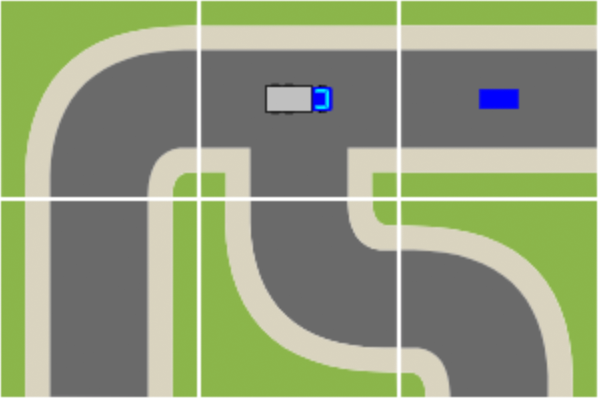
\includegraphics[width=\textwidth]{gfx/implementation-rendering-truck-position-diff-a.png}
    \caption{Haltepunkt auf der Mitte der Kachel}
    \label{fig:implementation:rendering:truck-position:diff:a}
  \end{subfigure}\hfill
  \begin{subfigure}[b]{0.45\textwidth}
    \includegraphics[width=\textwidth]{gfx/implementation-rendering-truck-position-diff-b.png}
    \caption{Haltepunkt auf der Kante der Kachel}
    \label{fig:implementation:rendering:truck-position:diff:b}
  \end{subfigure}\hfill
  \caption{Haltepunkte des Lastwagen im Spielfeld (zur besseren Erkennbarkeit sind die Kanten der Kacheln hervorgehoben)}
  \label{fig:implementation:rendering:truck-position:diff}
\end{figure}

\subsection{Animationsschritte}
\label{sec:implementation:rendering:animation}

Durch Animationen kann das Benutzererlebnis noch einmal deutlich aufgewertet werden, indem sie den Ausführungsfluss der Anwendung verlangsamen und dadurch die Nachvollziehbarkeit der ausgeführten Befehle ermöglicht wird. Zwischen den Positionen des Lastwagens wird daher zeitlich interpoliert. Eine wichtige Grundlage dafür wurde mit der Welt-Objektstruktur bereits geschaffen \tref{sec:implementation:structure}: Jede Operation erzeugt einen neuen Zustand, der in einer Liste gespeichert wird. Dieses Vorgehen macht es leicht zwischen dem aktuellen und dem vorherigen Zustand zu interpolieren.

Auch die in Abschnitt \ref{sec:implementation:evaluation:execution-time} beschriebenen Zeitschritte spielen an dieser Stelle eine wesentliche Rolle. Eine Animation der Bewegung des Lastwagens wird so z.~B. immer im Zeitraum eines Zeitschrittes animiert. Dadurch, dass die Ausführung des Programms genau diese Dauer als Ausführungszeit vorsieht, entsteht eine flüssige, nachvollziehbare Animation über mehrere Zeitschritte hinweg.

%************************************************
% Integration
%************************************************
\section[Integration]{Integration\protect\footnotemark}
\label{sec:implementation:integration}

\footnotetext{Zum Verständnis dieses Abschnittes werden grundlegende Kenntnisse über Angular (insbesondere Services und Komponenten) vorausgesetzt.}

Um mit möglichst wenigen Abhängigkeiten und dadurch geringerem Zeitaufwand verschiedene Ansätze ausprobieren zu können, wurde zunächst mit der Entwicklung eines Prototypen auf einer "grünen Wiese" begonnen. Auch wenn der Prototyp als Angular-Anwendung aufgesetzt wurde, erfolgte der Großteil der Entwicklung außerhalb dieser Umgebung. Nachdem der ursprüngliche Ansatz der Darstellung mittels SVG-Grafiken verworfen und die Darstellung auf Canvas-Rendering umgestellt wurde, sind die Objektstruktur, sowie der Renderer vollständig unabhängig von Angular implementiert, da sie von den von Angular bereitgestellten Strukturen nicht profitieren können. Diese Klassen konnten so ohne Anpassungen in die Umgebung von BlattWerkzeug übernommen werden. Lediglich die rudimentäre Benutzeroberfläche des Prototypen (siehe Abbildung \ref{fig:implementation:integration:prototype}) wurde mithilfe von Angular umgesetzt, für die Integration in BlattWerkzeug in dieser Form jedoch nicht mehr benötigt.

\begin{figure}
  \centering
  \includegraphics[width=0.4\textwidth]{gfx/implementation-integration-prototype.png}
  \caption{Bildschirmfoto der UI des Prototyp vor der Integration in BlattWerkzeug}
  \label{fig:implementation:integration:prototype}
\end{figure}

\subsection{Angular-Service}
\label{sec:implementation:integration:ng-service}

Ein Projekt in BlattWerkzeug kann sowohl mehrere Welten, als auch mehrere Programme beinhalten. Diese zusammenzubringen ist die Aufgabe des \inlinec{TruckWorldService}. Die Auslagerung dieser Funktionalität ist notwendig, da Darstellung und Steuerung der Welten über mehrere Angular-Komponenten verteilt sind. Alle diese Komponenten erhalten in Abhängigkeit des aktuell geöffneten Programmes die entsprechende Instanz der Welt. Auch übernimmt der Service die Aufgabe -- falls notwendig -- eine neue Instanz einer Welt zu erzeugen.

Eine besondere Schwierigkeit ist in diesem Zusammenhang die Zuordnung einer Welt zu einem Programm. BlattWerkzeug bietet aktuell nicht die Möglichkeit, eine Verknüpfung zwischen verschiedenen Ressourcen herzustellen. Zu diesem Zweck wurde eine Auswahlbox implementiert, welche in die UI der Controller-Komponente (siehe nächstes Kapitel) eingegliedert wurde und in einem Auswahlfeld alle im aktuellen Projekt verfügbaren Welten darstellt. Die Auswahl wird an den \inlinec{TruckWorldService} weitergegeben, der sie zwischenspeichert. So geht die Auswahl der Welt, sowie deren aktueller Zustand auch nicht verloren, wenn der Nutzer zwischen verschiedenen Programmen wechselt. Aufgrund der fehlenden Speichermöglichkeit in BlattWerkzeug, muss die Welt allerdings erneut ausgewählt werden, sobald die Seite neu geladen, und der Service dadurch neu instanziiert wird.

\subsection{Komponenten}
\label{sec:implementation:integration:components}

Innerhalb der UI von BlattWerkzeug werden die Funktionen dieser Erweiterung mithilfe von Komponenten dargestellt. Eine Übersicht der im Folgenden beschriebenen Komponenten findet sich in Abbildung \ref{fig:implementation:integration:components}.

An dieser Stelle soll bemerkt werden, dass die Sidebar, von der sich die einzelnen Befehle, Sensoren und anderen Elemente der Sprache in das Programm ziehen lassen, bewusst auf Deutsch gehalten ist, während die Befehle im Programm analog zu JavaScript in englischer Sprache gehalten sind. Dadurch soll der Nutzer von Anfang an mit dem Eindruck von Code vertraut gemacht werden, während er durch die deutschen Begriffe in Sidebar bei der Wahl der sprachlichen Elemente unterstützt wird.

\begin{figure}
  \centering
  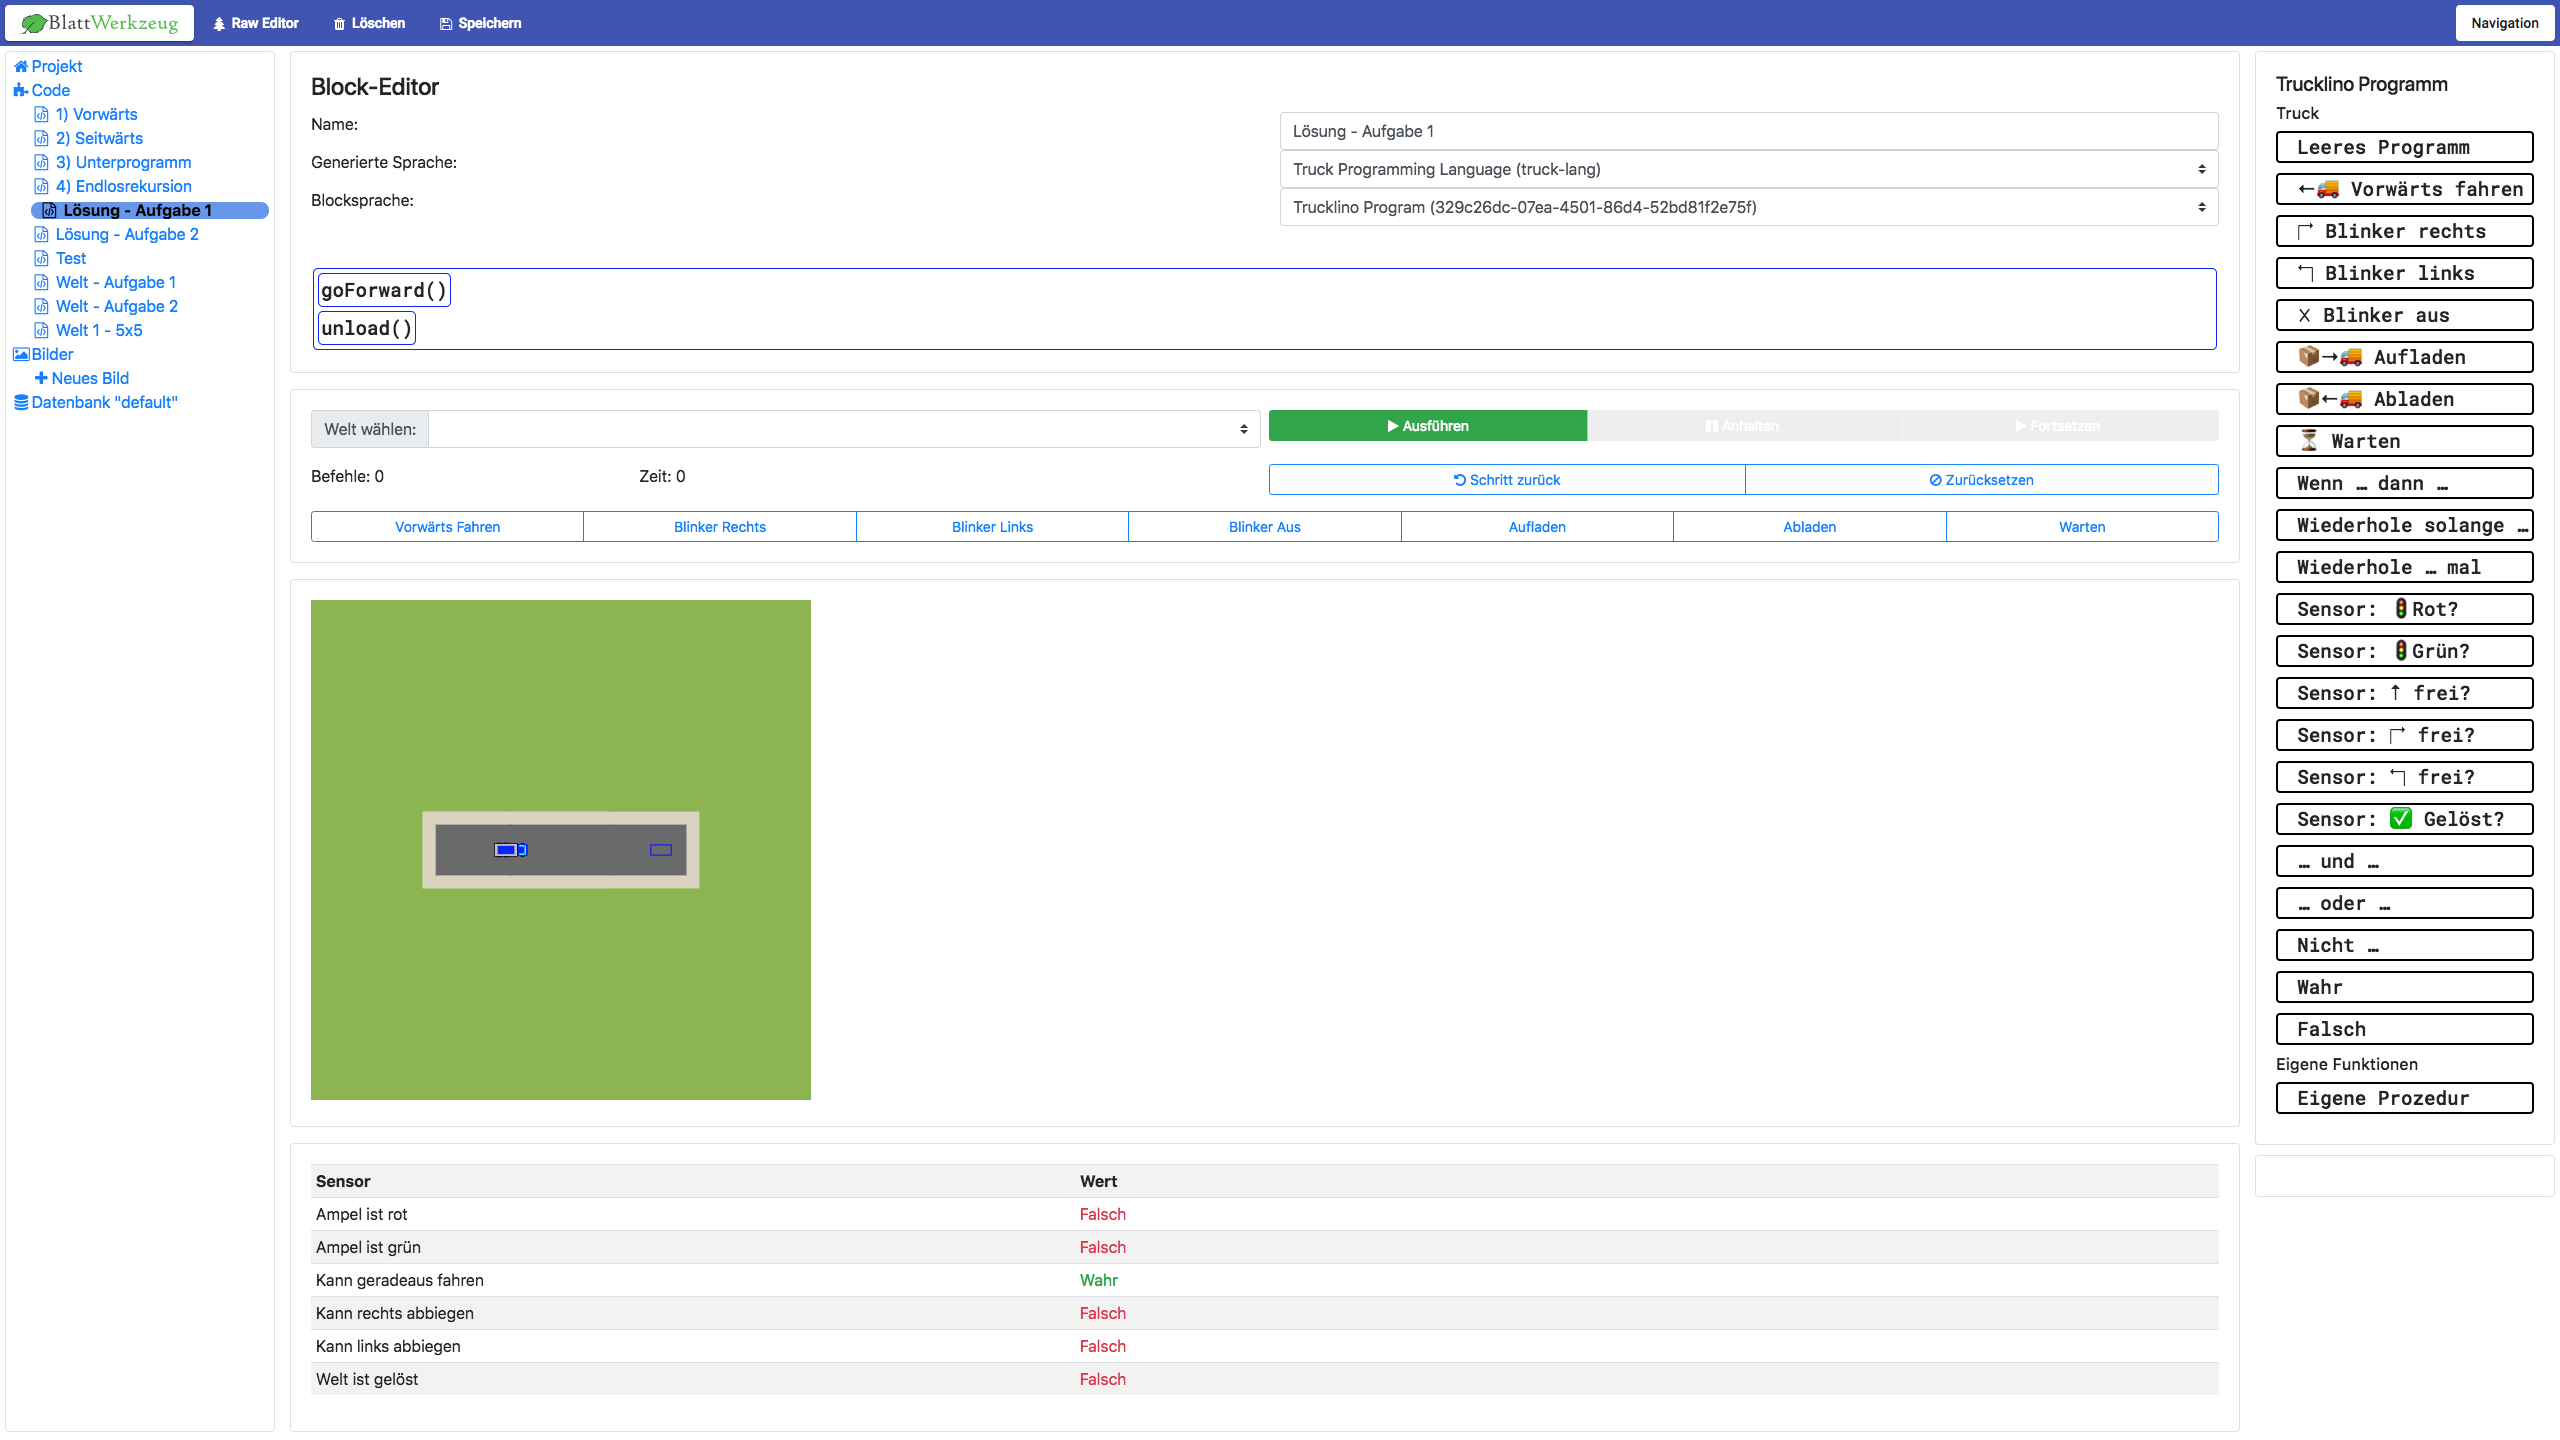
\includegraphics[width=1.0\textwidth]{gfx/implementation-integration-components.png}
  \caption{Bildschirmfoto der Komponenten in der UI von BlattWerkzeug}
  \label{fig:implementation:integration:components}
\end{figure}

\subsubsection{Renderer}
\label{sec:implementation:integration:renderer}

Zum Anzeigen der Welt wurde in BlattWerkzeug eine Komponente definiert, welche die \inlinec{Renderer}-Klasse (siehe \ref{sec:implementation:rendering:structure}) aus dem Prototypen nahezu ohne Anpassungen übernehmen konnte. Die Komponente erhält vom \inlinec{TruckWorldService} die aktuelle \inlinec{World}-Instanz, mit der sie den Renderer instanziiert und außerhalb der Angular Zone den Renderingprozess startet. Diese Komponente greift dabei lediglich lesend auf die Welt zu und nimmt keine Veränderungen vor.

Da der Renderingprozess bis zu 60 Mal in der Sekunde mittels \inlinec{requestAnimationFrame} ausgeführt wird, würde Angular andernfalls auch bis zu 60 Änderungserkennungen durchlaufen. Da keine Änderungen am Zustand vorgenommen werden, wäre dies in jedem Fall ergebnislos. Durch das Ausführen des Renderingprozesses außerhalb der Angular Zone, wird dies umgangen und die Performance kann gesteigert werden.

Zusätzlich wird die Komponente im Welt-Editor verwendet, um die bisher erstellte Welt darzustellen. Aus diesem Grund wurde darauf geachtet, die Darstellung möglichst robust und fehlertolerant zu gestalten, damit auch halb fertige Welten zuverlässig dargestellt werden können.

\subsubsection{Controller}
\label{sec:implementation:integration:controller}

Innerhalb der Controller-Komponente ist es möglich, die Befehle in der aktuellen Welt mithilfe von entsprechenden Buttons von Hand auszuführen. Außerdem kann an dieser Stelle die Ausführung des im Drag \& Drop-Editor zusammengestellten Programms gestartet und gestoppt werden. Es ist des Weiteren möglich, einzelne Befehle rückgängig zu machen oder die Welt direkt auf ihren Ausgangszustand zurückzusetzen.

Auch diese Komponente greift auf den \inlinec{TruckWorldService} zurück, um die aktuell gewählte Welt zu erhalten. Klicks auf die Buttons werden direkt an die entsprechenden Funktionen der \inlinec{World}-Klasse weitergeleitet.

Unter Verwendung des \inlinec{CurrentCodeResourceService}, einem von BlattWerkzeug bereitgestellten Service zum Erhalt der aktuellen Coderessource, kann auf den aus dem Drag \& Drop-Editor kompilierten Code zugegriffen werden. Dieser Code wird beim Klick auf den entsprechenden Button an die \inlinec{World}-Klasse zur Ausführung übergeben.

Solange eine Operation auf der Welt ausgeführt wird, sind die Bedienelemente zur Ausführung weiterer Befehle gesperrt. Erst nach Beendigung der Operation und damit auch der Animation, kann ein weiterer Befehl ausgeführt werden. Dazu existiert in der \inlinec{World}-Klasse ein Flag, welches während der Ausführung gesetzt und von dieser Komponente ständig ausgewertet wird.

\subsubsection{Sensoren}
\label{sec:implementation:integration:sensors}

Die Sensor-Komponente dient lediglich der Darstellung der aktuellen Werte aller Sensoren. Dadurch wird dem Nutzer im Navigationsmodus ermöglicht, sich in die Lage des Programms hineinzuversetzen und Entscheidungen basierend auf dem Wert von Sensoren zu treffen. Auch diese Komponente erhält über den \inlinec{TruckWorldService} Zugriff auf die aktuelle Welt, auf welche sie allerdings nur lesend zugreift.

%************************************************
% Zusammenfassung
%************************************************
\section{Zusammenfassung}
\label{sec:implementation:summary}

Dieses Kapitel beschreibt die Implementierung der im Rahmen dieser Arbeit entwickelten Erweiterung. In der Rahmenhandlung wird ein Lastwagen durch ein Netz von Straßen bewegt und löst Aufgaben, indem er farbige Container an ihre Ziele bringt.

Eine Objektstruktur verwaltet die Zustände der Mikrowelt, in der sich der Lastwagen bewegt. Gesteuert wird er durch den Nutzer mit Befehlen einer Minisprache, die mit ihrem reduzierten Umfang eine verständliche Einführung in verschiedene Konzepte wie Prozeduren, Schleifen und Verzweigungen gibt.

Die mit dem Drag \& Drop-Editor von BlattWerkzeug erstellten Programme werden in JavaScript Code übersetzt und die Ausführung in einer animierten Welt in einem Canvas-Element dargestellt. Ein zunächst entwickelter Prototyp wurde in Form eines Service und mehrerer Komponenten in das bestehende BlattWerkzeug-Projekt integriert.
